%% 
%% Copyright 2007-2024 Elsevier Ltd
%% 
%% This file is part of the 'Elsarticle Bundle'.
%% ---------------------------------------------
%% 
%% It may be distributed under the conditions of the LaTeX Project Public
%% License, either version 1.3 of this license or (at your option) any
%% later version.  The latest version of this license is in
%%    http://www.latex-project.org/lppl.txt
%% and version 1.3 or later is part of all distributions of LaTeX
%% version 1999/12/01 or later.
%% 
%% The list of all files belonging to the 'Elsarticle Bundle' is
%% given in the file `manifest.txt'.
%% 
%% Template article for Elsevier's document class `elsarticle'
%% with numbered style bibliographic references
%% SP 2008/03/01
%% $Id: elsarticle-template-num.tex 249 2024-04-06 10:51:24Z rishi $
%%
\documentclass[preprint,12pt]{elsarticle}
%% Use the option review to obtain double line spacing
%% \documentclass[authoryear,preprint,review,12pt]{elsarticle}

%% Use the options 1p,twocolumn; 3p; 3p,twocolumn; 5p; or 5p,twocolumn
%% for a journal layout:
%% \documentclass[final,1p,times]{elsarticle}
%% \documentclass[final,1p,times,twocolumn]{elsarticle}
%% \documentclass[final,3p,times]{elsarticle}
%% \documentclass[final,3p,times,twocolumn]{elsarticle}
%% \documentclass[final,5p,times]{elsarticle}
%% \documentclass[final,5p,times,twocolumn]{elsarticle}

%% For including figures, graphicx.sty has been loaded in
%% elsarticle.cls. If you prefer to use the old commands
%% please give \usepackage{epsfig}

%% The amssymb package provides various useful mathematical symbols
\usepackage{amssymb}
%% The amsmath package provides various useful equation environments.
\usepackage{amsmath}
%% The amsthm package provides extended theorem environments
%% \usepackage{amsthm}
%% i want to use bottem packges for make algorithm in latex
\usepackage{lineno}
\usepackage{algorithm}
\usepackage{algorithmic}
\usepackage[table,xcdraw]{xcolor}
\usepackage{multirow}
%%\usepackage{algpseudocode}
\begin{document}

\begin{frontmatter}

%% Title, authors and addresses

%% use the tnoteref command within \title for footnotes;
%% use the tnotetext command for theassociated footnote;
%% use the fnref command within \author or \affiliation for footnotes;
%% use the fntext command for theassociated footnote;
%% use the corref command within \author for corresponding author footnotes;
%% use the cortext command for theassociated footnote;
%% use the ead command for the email address,
%% and the form \ead[url] for the home page:
%% \title{Title\tnoteref{label1}}
%% \tnotetext[label1]{}
%% \author{Name\corref{cor1}\fnref{label2}}
%% \ead{email address}
%% \ead[url]{home page}
%% \fntext[label2]{}
%% \cortext[cor1]{}
%% \affiliation{organization={},
%%             addressline={},
%%             city={},
%%             postcode={},
%%             state={},
%%             country={}}
%% \fntext[label3]{}

\title{This is Title of my article}

%% use optional labels to link authors explicitly to addresses:
%% \author[label1,label2]{}
%% \affiliation[label1]{organization={},
%%             addressline={},
%%             city={},
%%             postcode={},
%%             state={},
%%             country={}}
%%
%% \affiliation[label2]{organization={},
%%             addressline={},
%%             city={},
%%             postcode={},
%%             state={},
%%             country={}}

\author{Mehrab Atighi , My Teachers} %% Author name

%% Author affiliation
\affiliation{organization={},%Department and Organization
            addressline={}, 
            city={},
            postcode={}, 
            state={},
            country={}}

%% Abstract
\begin{abstract}
%% Text of abstract
Abstract text.
\end{abstract}

%%Graphical abstract
%\begin{graphicalabstract}
%%\includegraphics{grabs}
%\end{graphicalabstract}
%
%%%Research highlights
%\begin{highlights}
%\item Research highlight 1
%\item Research highlight 2
%\end{highlights}

%% Keywords
\begin{keyword}
%% keywords here, in the form: keyword \sep keyword

%% PACS codes here, in the form: \PACS code \sep code

%% MSC codes here, in the form: \MSC code \sep code
%% or \MSC[2008] code \sep code (2000 is the default)

\end{keyword}

\end{frontmatter}

%% Add \usepackage{lineno} before \begin{document} and uncomment 
%% following line to enable line numbers
%% \linenumbers

%% main text
%%

%% Use \section commands to start a section
\section{INTRODUCTION}
\label{sec1}
%% Labels are used to cross-reference an item using \ref command.

Introduction text.


\section{RELATED WORKS  or LITERATURE REVIEW}
\label{sec2}
%% Labels are used to cross-reference an item using \ref command.
in this section i want to show the related works in 3 subset\\
first is Supervised and Unsupervised Learning Methods, \ref{sec2_1}.

second is ReSampling Methods, \ref{sec2_2}.

third is Metrics .
\ref{sec2_3}.


\subsection{Supervised and Unsupervised Learning Methods}
\label{sec2_1}
methods and refrences here


\subsection{Resampling Methods}
\label{sec2_2}
methods and refrences here


\subsection{Metrics}
\label{sec2_3}
methods and refrences here


\section{Available Methods}
\label{sec3}
i want to tell about the dimention reduction methods in \ref{sec3_1} ,
Outlier Detection methods in \ref{sec3_2} , 
Resampling method in \ref{sec3_3} , 
TYPES OF CLASSIFICATION ALGORITHMS in \ref{sec3_4} 
and usual usefull metrics in \ref{sec3_5}.

\subsection{dimention reduction methods}
\label{sec3_1}

Dimensionality reduction in machine learning refers to techniques that reduce the number of input variables (also known as features) in a dataset. When dealing with high-dimensional data, these methods project the data from a high-dimensional space into a lower-dimensional space while retaining the meaningful properties of the original data. The goal is to simplify the data representation, improve model performance, and mitigate the challenges posed by the “curse of dimensionality” when working with large feature sets.\\

in this section we are discuss about the Gini index in \ref{sec3_1_1} and NearZeroVariance method in \ref{sec3_1_2}

\subsubsection{Gini Index}
\label{sec3_1_1}

Gini Index for Categorical Columns: Assume Y is a categorical response, and the covariate matrix X is a multivariate covariate matrix of $n \times P$ dimension with G grouped covariates. $X_g$ represents the g-th group covariate, $p_g$ represents the dimension of the covariates in the g-th group covariates. All the covariate components of the covariate matrix X are classified with J categories. The values of any element in $$X_g \in {1, … ,J}$$, $J_p_g$ combinations were formed.\\
The marginal Gini impurity of Y is defined as $$Gini(Y) = 1 -  \sum_{}^{}Pr^2$$ from r=1 to R. The Gini index is a value between 0 and 1, where 0 means that all observations are the same. The closer it is to 0, the more equal the observations are, and the closer it is to 1, the more different the observations are.

\subsubsection{Near Zero Variance Method}
\label{sec3_1_2}
The nearZeroVar function identifies predictors that have one unique value (zero variance predictors) or predictors that have very few unique values relative to the number of samples and a large ratio of the frequency of the most common value to the frequency of the second most common value. For instance, a predictor with two distinct values out of 1000 samples, where 999 of them are a single value, is considered a near zero variance predictor. To be flagged, the frequency ratio must be above freqCut, and the percent of unique values must be below uniqueCut. The default value for freqCut is 95.5 and uniqueCut is 10.


\subsection{Outlier Detection methods}
\label{sec3_2}

in this section we are discuss about the 

Box plot method in \ref{sec3_2_1},
Percentile method in \ref{sec3_2_2},
ZScore method in \ref{sec3_2_3},
Hample filter method in \ref{sec3_2_4},
E-Grubs test method in \ref{sec3_2_5},
Local outlier factor method in \ref{sec3_2_6},
Knn method in \ref{sec3_2_7},
Isolation forest method in \ref{sec3_2_8} and
KModes method in \ref{sec3_2_9}.


\subsubsection{Box plot method}
\label{sec3_2_1}
Detect outliers using boxplot methods. Boxplots are a popular and an easy method for identifying outliers.
There are two categories of outlier: (1) outliers and (2) extreme points.
Values above  $Q3 + (1.5 \times IQR)$ or below Q1 - (1.5 \times IQR) are considered as outliers. Values above 
$Q3 + (3 \times IQR)$ or below  $Q1 - (3 \times IQR)$ are considered as extreme points (or extreme outliers).
Q1 and Q3 are the first and third quartile, respectively.\\
IQR is the interquartile range $(IQR = Q_3 - Q_1)$.

\subsubsection{Percentile method}
\label{sec3_2_2}
Percentiles are a useful tool for identifying outliers in a dataset. Percentiles divide the data into 100 equal parts, and the value at each percentile indicates the number below which a certain percentage of the data falls. For example, the value at the $25_th$ percentile is the number below which $25\%$ of the data falls, and the value at the $75_th$ percentile is the number below which $75\%$ of the data falls. In this article we flag data as
outlier when they are lower than percentile $5\%$ and more than percentile $95\%$ in other words the normal data are between $(5 , 95) \%$ percentiles that include $90\%$ of data.

\subsubsection{ZScore method}
\label{sec3_2_3}
Another method that can be used to screen data for outliers is the Z-Score, using the mean and
standard deviation.
$Z_i = X_i  - \bar{X}$
$sd$ , where $X_i  \thicksim N(\mu, \sigma ^ 2)$, and $sd$ is the standard deviation of data.\\
The basic idea of this rule is that if 𝑋 follows a normal distribution, $N(\mu, \sigma ^ 2)$, then 𝑍 follows a standard normal distribution, $N(0, 1)$, and Zscores that exceed 3 in absolute value are generally considered as outliers. This method is simple and it is the same formula as the 3 SD method when the criterion of an outlier is an absolute value of a Z-score of at least 3. It presents a reasonable criterion for identification of the outlier when data follow the normal distribution.

\subsubsection{Hample filter method}
\label{sec3_2_4}
The Hampel Identifier is a method that recognizes isolated outliers. It uses the median and median absolute deviation as a robust estimate of the location and spread of the outliers. The Hampel identifier is defined for data sequences $x_1, x_2, …, x_n$ with a moving window length of 2k + 1, and the local median is $m_i$.\\
The scale estimate of median estimated deviation (MADse) is Si. When the difference between the measured data and the local median is greater than t times MADse, the measured value is considered to be an outlier. The value of t is generally 3. When t = 0, then $y_i = m_i$, the Hampel identifier becomes the standard median filter.

\subsubsection{E-Grubs test method}
\label{sec3_2_5}
The Grubbs’ test is a statistical method used to detect outliers in a univariate data set that follows a normal distribution. It operates under two hypotheses: no outliers ($H_0$) and exactly one outlier ($H_1$). The test uses the sample mean and standard deviation to calculate a test statistic, which is then compared to a critical value to determine the presence of an outlier.

\subsubsection{Local outlier factor method}
\label{sec3_2_6}
The Local Outlier Factor ($LOF$) is a density-based clustering method for detecting outliers, using the $K-Nearest Neighbor$ ($KNN$) technique. It measures local reachability density (lrd) to differentiate each point with its neighborhood. The $LOF$ score increases for an observation if its lrd value is less than the estimated nearest neighbor. A $simplifiedLOF$ method was introduced to make density estimation simpler, adopting $KNN$ distance instead of $LOF$’s reachability distance. Although more computationally complex, the $simplifiedLOF$ improves performance.

\subsubsection{Knn method}
\label{sec3_2_7}

A high-level summary of the nearest neighbor classification method is given in Algorithm KNN. The algorithm computes the distance (or similarity) between each test instance $z = (x,y)$ and all the training examples $(x,y) \in D $ to determine its nearest neighbor list, $D_z$. Such computation can be costly if the number of training examples is large. However, efficient indexing techniques are available to reduce the computation needed to find the nearest neighbors
of a test instance.\\

\begin{algorithm}
	\caption{The K-nearest neighbor classifier}\label{your_label}
	\begin{algorithmic}
		\STATE  Let k be the number of nearest neighbors and D be the set of traning examples.
		\FOR{each test instance $z = (x',y')$ do}
		\STATE Compute $d(x^\prime, x )$, the distance between z and every example , $(x,y)\in D$
		\STATE Select $D_z\subseteq D$, the set of k closest traning examples to z.
		\STATE $y^\prime={\rm argmax}\nu{\sum_{\left(x_i,y_i\right)\in D_z} I\left(\nu=y_i\right)}$
		\ENDFOR
	\end{algorithmic}
\end{algorithm}



\subsubsection{Isolation forest method}
\label{sec3_2_8}
The $Isolation Forest(iForest)$ is applied to initially process the dataset, aiming at mining outlier candidates. It is an ensemble-based unsupervised outlier detection method with linear time complexity and high precision. The forest consists of a group of binary trees constructed from the random property of the dataset. Then, traverse each tree in the forest and calculate the anomaly score of each data point in each tree. The isolation tree’s construction algorithm is defined as $iTree\ (X,\ e,\ h)$ function. Here, X represents the input dataset, e represents the current tree height, h\ represents height limit. The steps of the iForest’s construction algorithm are as follows: 

\begin{algorithm}
	\caption{Isolation Forest $(X,t,s)$}\label{your_label}
	\begin{algorithmic}
	\STATE \textbf{Input:} X- input dataset , t – number of trees , s – subsampling size.
	\STATE \textbf{Output:} a set of t iTrees.
	\STATE 1: Initialize Forest 
	\STATE 2: set height limit $l=ceilinglog_2\ s$
	\FOR {i = $1$ to $t$}
	\STATE $X\prime = sample(X , s)$
	\STATE $Forest = Forest \cup (iTree , 0 , l)$
	\ENDFOR
	\RETURN Forest

	\end{algorithmic}
\end{algorithm}


\subsubsection{KModes method}
\label{sec3_2_9}
The K − modes clustering algorithm was proposed as an alternative to the popular K − means algorithm, the most used centroid-based non-hierarchical algorithm. The K − modes (Algorithm 1) algorithm begins with a random selection of k objects (centroids) which are the central objects of k clusters. Then, the dissimilarity measure is calculated and the closest centroid is determined for each object. When all objects are assigned to individual clusters, the centroids are updated by creating new modes from objects present in the cluster. The calculations are repeated until the differences in the generated clusters in the following steps cease to exist.

\begin{algorithm}
	\caption{K Modes}\label{your_label}
	\begin{algorithmic}
		\STATE Randomly select k items (modes) from the dataset.
		\FOR {each pair (Mode , Object)}
		\STATE calculate the dissimilarity measure.
		\ENDFOR
		\WHILE{the generated clusters do not repeat themselves.}
		\FOR {each object that is not a mode}
		\STATE find the mode closest to the object.
		\ENDFOR
		\STATE Join object with the corresponding modes to create clusters.
		\FOR {All Clusters}
		\STATE recalculate the modal vectors containing in successive coordinate the most common values on attributes of cluster objects.
		\ENDFOR
		\ENDWHILE
	
\end{algorithmic}
\end{algorithm}


\subsection{Resampling methods}
\label{sec3_3}
in this section i want to describe Random oversampling method in \ref{sec3_3_1}


\subsubsection{Random oversampling method}
\label{sec3_3_1}
Random Over-Sampling is a technique based on bootstrap that supports the binary classification task in the presence of unbalanced classes by generating synthetic examples from a conditional density estimation of the two classes. It handles both continuous and categorical data. By repeating the original samples, as a result of this process, the dataset grows in size. The argument is that no new samples are generated by a random over-sampler, and the variety of samples remains constant.



\subsection{TYPES OF CLASSIFICATION ALGORITHMS}
\label{sec3_4}


in this section i want to descuss about the type of classification algorithms 
LR models in \ref{sec3_4_1} , 
SVM models in \ref{sec3_4_2} ,  
XGB models in \ref{sec3_4_3} , 
RF models in \ref{sec3_4_4} , 
NB models in \ref{sec3_4_5} , 
KNN models in \ref{sec3_4_6} , 
ADAB Boost models in \ref{sec3_4_7} and 
NN models in \ref{sec3_4_8}.


\subsubsection{LR models}
\label{sec3_4_1}
 Logistic Regression (LR) is a widely used supervised learning model. It predicts outcomes based on input features and target variables. In binomial logistic regression, we calculate the linear relationship between variables using the logit function. The sigmoid curve restricts LR’s output between 0 and 1. LR’s goal is to find optimal parameters $((\beta_0) and (\beta_i))$ by maximizing log-likelihood. It’s commonly used for binary classification tasks, such as fraud detection, where we set a threshold © to classify predictions .

\subsubsection{SVM models}
\label{sec3_4_2}
The SVM is a popular machine learning classifier that is used in our research. It is being applied for both
linear and nonlinear problems in real-world domain areas . A hyperplane is used to separate instances
of classes in SVM. Because of its kernel function which is used to convert low dimension space to high dimension space SVM is best suited for nonlinear classification problems. Summarizing we can say that SVM can be used for classifying instances in complex problems in an efficient way


\subsubsection{XGB models}
\label{sec3_4_3}
XGBoost, an efficient gradient boosting implementation, constructs additive models using decision trees. By iteratively minimizing errors, it creates an ensemble of base learners that outperform individual classifiers. XGBoost enhances accuracy, controls overfitting, and incorporates stochastic gradient boosting. Its objective function balances prediction quality and model complexity. Successfully applied in various domains, XGBoost is particularly effective for detecting insurance fraud in high-dimensional data . 

\subsubsection{RF models}
\label{sec3_4_4}
Leo Breiman and Adèle Cutler proposed the RF classifier in 2001. It works by utilizing the combined effect of two concepts “bagging” and “subspaces”.From the training dataset, a set of decision trees are built and decision i.e. label is predicted based on votes collected from these decision tresses. RF provides high accuracy and is mainly used for classifying large datasets due to its ability to handle missing values. The application domains of RF include remote sensing, e-commerce, stock market, fraud detection, network intrusion detection, and so on.

\subsubsection{NB models}
\label{sec3_4_5}
Naïve Bayes (NB) is a powerful model for predicting test accuracy in large datasets. It leverages Bayes’ theorem, assuming independence between predictors. In fraud detection, NB treats attribute existence within a class as irrelevant to other attributes. By using the naïve assumption of conditional independence, it efficiently identifies fraudulent patterns. The model calculates probabilities using Maximum A Posteriori (MAP) and distinguishes itself by its assumptions about the distribution of features .

\subsubsection{KNN models}
\label{sec3_4_6}
We discussed about this method in above\ref{sec3_2_7}.

\subsubsection{ADAB Boost models}
\label{sec3_4_7}
Adaboost which is also called Adaptive Boosting. This algorithm is famous for its quick boosting in machine learning. Boosting algorithms are very suitable for transforming a lazy learner into an eager learner. The basic purpose of adaptive boosting is to enhance the predictive ability of lazy learners with the help of training. To have a strong learner Adaboost merges many weak and slow learners. At the start of the algorithm weights of each attribute are identical and by the further run of the algorithm, weights start to update.

\subsubsection{NN models}
\label{sec3_4_8}
Neural networks are powerful models inspired by the human brain. They learn patterns from data and make predictions. These networks consist of interconnected artificial neurons that process information layer by layer. By adjusting weights and biases, neural networks adapt to complex relationships in the data. Deep learning, a subset of neural networks, has revolutionized fields like image recognition, natural language processing, and fraud detection. Understanding neural networks is essential for unlocking their potential in solving real-world problems.



\subsection{usefull metrics}
\label{sec3_5}




in this section i want to discuss about the type of mterics for evaluate models.
Accuracy/Weighted Recall metric in \ref{sec3_5_1},
Area Under Receiver Operating Characteristic Curve (AUC-ROC) metric in \ref{sec3_5_2},
Balanced Accuracy metric in \ref{sec3_5_3},
F1-score  metric in \ref{sec3_5_4},
Brier Score loss metric in \ref{sec3_5_5},
Precision metric in \ref{sec3_5_6},
Recall/Sensitivity  metric in \ref{sec3_5_7} and
Specificity  metric in \ref{sec3_5_8}.

\subsubsection{Accuracy/Weighted Recall metric}
\label{sec3_5_1}
The accuracy is defined as the ratio of correctly predicted to total number of instances; it is calculated using the following formula:
$$Acc=\frac{TP+TN}{TP+TN+FP+FN}$$
where TP and TN are the number of correctly predicted positives and negatives, respectively, while FP and FP are the number of falsely predicted positives and negatives, respectively.


\subsubsection{Area Under Receiver Operating Characteristic Curve (AUC-ROC) metric}
\label{sec3_5_2}
ROC AUC score is the area under the ROC curve; it quantifies the ability of the model to distinguish between positive and negative classes

\subsubsection{Balanced Accuracy metric}
\label{sec3_5_3}
Balanced accuracy is defined as the average of recall and precision; it is calculated using the following formula:
$$BAcc=\frac{RS+PS}{2}$$

\subsubsection{F1-score  metric}
\label{sec3_5_4}
F1-score is defined as the harmonic mean of precision and recall; it is calculated using the following formula
$$F1=\frac{2\times P S\times R S}{PS+RS}$$

\subsubsection{Brier Score loss metric}
\label{sec3_5_5}
Brier score loss is a proper scoring rule which quantifies the accuracy of probabilistic predictions; it is calculated using the following formula:
$$BSL=\frac{1}{N}\sum_{i=1}^{N}\left(y_i-\ \widehat{y_i}\right)^2$$
where $\widehat{y_i}$is the predicted probability of the i-th instance being positive and $y_i$ is its actual class label.


\subsubsection{Precision metric}
\label{sec3_5_6}
Precision is defined as the ratio of correctly predicted positive instances to the total number of predicted positive instances; it is calculated using the following formula:
$$PS=\frac{TP}{TP+FP}$$


\subsubsection{Recall/Sensitivity  metric}
\label{sec3_5_7}
Recall is defined as the ratio of correctly predicted positive instances
to the total number of positive instances; it is calculated using the following formula:
$$RS\ or\ Recall\ Score=\frac{TP}{FP+TN}$$
where TP and FN are the numbers of true positive and false negative transactions.



\subsubsection{Specificity  metric}
\label{sec3_5_8}

 Specificity (true negative rate) is the probability of a negative test result, conditioned on the individual truly being negative.\\
$$Specifity=\frac{TN}{TN=FP}$$



\section{PROPOSED ALGORITHM}
\label{sec4}

This is all of my algs.
ALL OF WORK alg in \ref{sec4_1},
PreProcessing Alg in \ref{sec4_2},
Labeling method simple alg in \ref{sec4_3} and
Machine Learnin Part alg in \ref{sec4_4}.

\subsection{ALL OF WORK alg}
\label{sec4_1}
this algorithm is speak about all of our work
\begin{algorithm}
	\caption{All of Work}\label{algo:allofwork}
	\begin{algorithmic}
		\STATE \textbf{STEP 1 PreProcessing:}
		\STATE Spliting Data Into Separate Partitions.
		\STATE \textbf{STEP 2 Labeling:}
		\STATE Use outlier or anomaly or fraud detection methods for labeling the observation as fraud or not.
		\STATE \textbf{STEP 3 Machine Learning:}
		\STATE Learn Machine Learning models.
		\STATE \textbf{STEP 4 Dynamic model update:}
		\STATE Learn Machine Learning models.
		\WHILE {the new part of data is available }
		\FOR {each learned ml models}
		\STATE Classification on the new part of dataset.
		\ENDFOR
		\FOR {each row of part of data}
		\STATE We will Count the classification labeld into number of fraud detected.
		\IF {number of voting \lq fraud detected}
			\STATE Label case as fraud
			\ELSE 
			\STATE Label case as normal.
		\ENDIF
		\STATE 	Send suspicious(fraud detected) case into expert for get their feedback.
		\IF {suspicious case labeled wrong}
			\STATE the expert will send a feedback to edit the case label.
		\ELSE 
		\STATE the data is Okey.
		\ENDIF
		\ENDFOR
		\ENDWHILE
		\STATE \textbf{Go To Step 3}	
	\end{algorithmic}
\end{algorithm}


\subsection{PreProcessing Alg}
\label{sec4_2}

this algorithm is speak about PreProcessing Step of our work
\begin{algorithm}
	\caption{PreProcessing}\label{algo:preprocessing}
	\begin{algorithmic}
		\STATE We do a random sample to move the cases.
		
		\FOR {each categorical column}
		\STATE Use gini index method for feature selection.
		\IF { the column is not good }
		\STATE remove column.
		\ELSE 
		\STATE save column.
		\ENDIF
		\ENDFOR
		
		\FOR {each numerical column}
		\STATE Use NearZeroVariance method for feature selection.
		\IF { the column is not good }
		\STATE remove column.
		\ELSE 
		\STATE save column.
		\ENDIF
		\ENDFOR
		\STATE Separate the Dataset into 4 partition as follow
		\STATE \textbf{Part 1)} from 1 to percent 1 rows of dataset.
		\STATE \textbf{Part 2)} from percent 1 + 1 to percent 2 rows of dataset.
		\STATE \textbf{Part 3)} from percent 2 + 1 to percent 3 rows of dataset.
		\STATE \textbf{Part 4)} from percent 3 + 1 to percent 4 rows of dataset.
		
	\end{algorithmic}
\end{algorithm}

\subsection{Labeling method simple alg}
\label{sec4_3}

this algorithm is speak about simple \textbf{Labeling} method Step of our work
\begin{algorithm}
\caption{Labeling}\label{algo:labeling}
\begin{algorithmic}
	\STATE \textbf{Numerical Outlier detection methods:} box-plot, percentile, Z-Score, Hampel filter, E-Grubs test, Local outlier factor, isolation forest.
	\STATE \textbf{Categorical Outlier detection methods:} K-Modes.
	
	\FOR{each numerical column of part 1}
	\FOR{each row of data}
	\STATE Use numerical outlier detection methods.
	\STATE Save 8 binary results (votes) for each row.
	\ENDFOR
	\ENDFOR
	
	\FOR{each categorical column of part 1}
	\FOR{each row of data}
	\STATE Use categorical outlier detection methods.
	\STATE Save 1 binary result (vote) for each row.
	\ENDFOR
	\ENDFOR
	
	\FOR{each row of part 1}
	\STATE \textbf{Count} the outlier detection results.
	\IF{outlier detected $\geq$ number of votes}
	\STATE Label case as fraud.
	\ELSE
	\STATE Label case as normal.
	\ENDIF
	\ENDFOR
\end{algorithmic}
\end{algorithm}

\subsection{Machine Learnin Part alg}
\label{sec4_4}

this algorithm is speak about simple \textbf{Machine Learning and Dynamic model update} Steps of our work.
\begin{algorithm}
	\caption{Machine Learnin}\label{algo:machinelearning}
	\begin{algorithmic}
		\STATE $J \gets 1$
		\WHILE{part $J$ is available}
		\STATE Get random sample of partition $j$ from all fraud-labeled rows
		\STATE Union this sample with 10\% of normal rows to create Train $J$ dataset (union of partitions up to $j$)
		\STATE Use SMOTE method for balancing the Train $J$ dataset
		\FOR{each machine learning model}
		\STATE Learn ML model with Train $J$ dataset
		\ENDFOR
		\STATE $J \gets J + 1$
		\FOR{each row of part $J$}
		\FOR{each learned models}
		\STATE Prediction of classification on the row and save a binary result (fraud or not)
		\ENDFOR
		\IF{count of fraud results $\geq$ model\_num}
		\STATE Label row as fraud
		\STATE Send row to expert
		\IF{expert disagrees with fraud result}
		\STATE Update row label
		\ELSE
		\STATE Row labeled TRUE
		\ENDIF
		\ELSE
		\STATE Label row as normal data
		\ENDIF
		\ENDFOR
		\ENDWHILE
		\STATE You have the final model and it's ready for new cases
	\end{algorithmic}
\end{algorithm}


\section{DataSets}
\label{sec5}
in this section i want to discuss about used datasets.

Carclaims dataset in \ref{sec5_1},
fraud oracle  in \ref{sec5_2} and
insurance fraud claim in \ref{sec5_3}.


\subsection{Carclaims dataset}
\label{sec5_1}
whats the  Carclaims dataset?


\subsection{fraud oracle}
\label{sec5_2}
whats the  fraud oracle?


\subsection{insurance fraud claim}
\label{sec5_3}
whats the  insurance fraud claim?



\section{Experimental Results}
\label{sec6}

at the first we will show tables of times\ref{times_section} then modeling evaluation\ref{metrics_section}.

\subsection{Times Tables}\label{times_section}
this is the accuracy table here:

\begin{table}[ht]
	\centering
		\resizebox{\textwidth}{!}{%
	\begin{tabular}{rlrllllllll}
		\hline
		\multicolumn{2}{|c|}{Dataset name} & \multicolumn{4}{|c|}{carclaims} & \multicolumn{4}{|c|}{fraud oracle}  \\ 
		\hline
		 \multicolumn{1}{|c|}{Model Name} & \multicolumn{1}{|c|}{Round number}   & Accuracy & F1 & Recall & \multicolumn{1}{c|}{Sensitivity} & Accuracy & F1 & Recall & \multicolumn{1}{c|}{Sensitivity} \\ \hline
		 \multicolumn{1}{|c|}{adab} & \multicolumn{1}{|c|}{1} & 0.754 & 0.856 & 0.787 & \multicolumn{1}{c|}{0.787} & 0.793 & 0.883 & 0.833 & \multicolumn{1}{c|}{0.833} \\ \cline{1-2}
		 \multicolumn{1}{|c|}{adab} & \multicolumn{1}{|c|}{2} & 0.748 & 0.852 & 0.777 & \multicolumn{1}{c|}{0.777} & 0.736 & 0.846 & 0.770 & \multicolumn{1}{c|}{0.770} \\ \cline{1-2}
		 \multicolumn{1}{|c|}{adab} & \multicolumn{1}{|c|}{3} & 0.740 & 0.848 & 0.771 & \multicolumn{1}{c|}{0.771} & 0.789 & 0.881 & 0.825 & \multicolumn{1}{c|}{0.825} \\ \cline{1-2}
		 \multicolumn{1}{|c|}{knn} & \multicolumn{1}{|c|}{1} & 0.690 & 0.812 & 0.717 & \multicolumn{1}{c|}{0.717} & 0.714 & 0.830 & 0.745 & \multicolumn{1}{c|}{0.745} \\ \cline{1-2}
		 \multicolumn{1}{|c|}{knn} & \multicolumn{1}{|c|}{2} & 0.718 & 0.833 & 0.747 & \multicolumn{1}{c|}{0.747} & 0.723 & 0.837 & 0.753 & \multicolumn{1}{c|}{0.753} \\ \cline{1-2}
		 \multicolumn{1}{|c|}{knn} & \multicolumn{1}{|c|}{3} & 0.755 & 0.858 & 0.790 & \multicolumn{1}{c|}{0.790} & 0.759 & 0.861 & 0.792 & \multicolumn{1}{c|}{0.792} \\ \cline{1-2}
		 \multicolumn{1}{|c|}{ml} & \multicolumn{1}{|c|}{1} & 0.802 & 0.889 & 0.844 & \multicolumn{1}{c|}{0.844} & 0.796 & 0.885 & 0.840 & \multicolumn{1}{c|}{0.840} \\ \cline{1-2}
		 \multicolumn{1}{|c|}{ml} & \multicolumn{1}{|c|}{2} & 0.794 & 0.884 & 0.830 & \multicolumn{1}{c|}{0.830} & 0.811 & 0.895 & 0.848 & \multicolumn{1}{c|}{0.848} \\ \cline{1-2}
		 \multicolumn{1}{|c|}{ml} & \multicolumn{1}{|c|}{3} & 0.820 & 0.901 & 0.858 & \multicolumn{1}{c|}{0.858} & 0.814 & 0.897 & 0.850 & \multicolumn{1}{c|}{0.850} \\ \cline{1-2}
		 \multicolumn{1}{|c|}{nb} & \multicolumn{1}{|c|}{1} & 0.831 & 0.907 & 0.875 & \multicolumn{1}{c|}{0.875} & 0.827 & 0.905 & 0.872 & \multicolumn{1}{c|}{0.872} \\ \cline{1-2}
		 \multicolumn{1}{|c|}{nb} & \multicolumn{1}{|c|}{2} & 0.809 & 0.893 & 0.848 & \multicolumn{1}{c|}{0.848} & 0.811 & 0.894 & 0.850 & \multicolumn{1}{c|}{0.850} \\ \cline{1-2}
		 \multicolumn{1}{|c|}{nb} & \multicolumn{1}{|c|}{3} & 0.833 & 0.909 & 0.875 & \multicolumn{1}{c|}{0.875} & 0.838 & 0.912 & 0.877 & \multicolumn{1}{c|}{0.877} \\ \cline{1-2}
		 \multicolumn{1}{|c|}{nn} & \multicolumn{1}{|c|}{1} & 0.780 & 0.875 & 0.818 & \multicolumn{1}{c|}{0.818} & 0.823 & 0.903 & 0.868 & \multicolumn{1}{c|}{0.867} \\ \cline{1-2}
		 \multicolumn{1}{|c|}{nn} & \multicolumn{1}{|c|}{2} & 0.821 & 0.902 & 0.865 & \multicolumn{1}{c|}{0.865} & 0.835 & 0.910 & 0.878 & \multicolumn{1}{c|}{0.878} \\ \cline{1-2}
		 \multicolumn{1}{|c|}{nn} & \multicolumn{1}{|c|}{3} & 0.817 & 0.899 & 0.856 & \multicolumn{1}{c|}{0.856} & 0.786 & 0.879 & 0.820 & \multicolumn{1}{c|}{0.820} \\ \cline{1-2}
		 \multicolumn{1}{|c|}{rf} & \multicolumn{1}{|c|}{1} & 0.862 & 0.926 & 0.914 & \multicolumn{1}{c|}{0.914} & 0.870 & 0.930 & 0.922 & \multicolumn{1}{c|}{0.922} \\ \cline{1-2}
		 \multicolumn{1}{|c|}{rf} & \multicolumn{1}{|c|}{2} & 0.893 & 0.942 & 0.941 & \multicolumn{1}{c|}{0.941} & 0.889 & 0.940 & 0.937 & \multicolumn{1}{c|}{0.937} \\ \cline{1-2}
		 \multicolumn{1}{|c|}{rf} & \multicolumn{1}{|c|}{3} & 0.920 & 0.957 & 0.970& \multicolumn{1}{c|}{0.970} & 0.917 & 0.956 & 0.966 & \multicolumn{1}{c|}{0.966} \\ \cline{1-2}
		 \multicolumn{1}{|c|}{svm} & \multicolumn{1}{|c|}{1} & 0.791 & 0.881 & 0.830 & \multicolumn{1}{c|}{0.830} & 0.794 & 0.884 & 0.833 & \multicolumn{1}{c|}{0.833} \\ \cline{1-2}
		 \multicolumn{1}{|c|}{svm} & \multicolumn{1}{|c|}{2} & 0.791& 0.882 & 0.830 & \multicolumn{1}{c|}{0.830} & 0.801 & 0.888 & 0.837 & \multicolumn{1}{c|}{0.837} \\ \cline{1-2}
		 \multicolumn{1}{|c|}{svm} & \multicolumn{1}{|c|}{3} & 0.817 & 0.899 & 0.852 & \multicolumn{1}{c|}{0.852} & 0.815 & 0.897 & 0.850 & \multicolumn{1}{c|}{0.850} \\  \cline{1-2}
		 \multicolumn{1}{|c|}{xgb} & \multicolumn{1}{|c|}{1} & 0.813 & 0.896 & 0.856 & \multicolumn{1}{c|}{0.856} & 0.854 & 0.916 & 0.894 & \multicolumn{1}{c|}{0.894} \\ \cline{1-2}
		 \multicolumn{1}{|c|}{xgb} & \multicolumn{1}{|c|}{2} & 0.828 & 0.906 & 0.871 & \multicolumn{1}{c|}{0.871}  & 0.857 & 0.923 & 0.905 & \multicolumn{1}{c|}{0.905} \\ \cline{1-2}
		 \multicolumn{1}{|c|}{xgb} &\multicolumn{1}{|c|}{3} & 0.812 & 0.896 & 0.852 & \multicolumn{1}{c|}{0.852} & 0.860 & 0.924 & 0.900 & \multicolumn{1}{c|}{0.900} \\ \cline{1-2}
		 \multicolumn{1}{|c|}{total} & \multicolumn{1}{|c|}{1} & 0.879 & 0.935 & 0.934 & \multicolumn{1}{c|}{0.934} &  0.891 & 0.941 & 0.946 & \multicolumn{1}{c|}{0.946} \\ \cline{1-2}
		 \multicolumn{1}{|c|}{total} & \multicolumn{1}{|c|}{2} & 0.892 & 0.942 & 0.941 & \multicolumn{1}{c|}{0.941} & 0.895 & 0.943 & 0.943 & \multicolumn{1}{c|}{0.943} \\ \cline{1-2}
		 \multicolumn{1}{|c|}{total} & \multicolumn{1}{|c|}{3} & 0.941 & 0.970 & 0.995 & \multicolumn{1}{c|}{0.995} & 0.938 & 0.968 & 0.991 & \multicolumn{1}{c|}{0.991} \\ \cline{1-2}
		\hline
	\end{tabular}
}
\end{table}



\subsection{Times Tables}\label{metrics_section}
\begin{table}[ht]
	\resizebox{\textwidth}{!}{%
	\centering
	\begin{tabular}{rlrrrrrrrrrr}
		\hline
		\multicolumn{2}{|l|}{\cellcolor[HTML]{656565}{\color[HTML]{FFFFFF} Accuracy}}& \multicolumn{5}{|c|}{carclaims}  & \multicolumn{5}{|c|}{fraud oracle}  \\ \cline{1-12}
		%\hline
		\multicolumn{2}{|l|}{Model Num \textbackslash Vote num}  & 1 & 2 & 3 & 4 & 5 & 1 & 2 & 3 & 4 & \multicolumn{1}{c|}{5}   \\ \cline{1-2}
		\hline
		\multicolumn{2}{|l|}{3} & 0.448 & 0.429 & 0.687 & 0.720 & 0.793 & 0.417 & 0.388 & 0.690 & 0.763 & \multicolumn{1}{c|}{0.775}  \\ \cline{1-2}
		\multicolumn{2}{|l|}{4} & 0.565 & 0.534 & 0.766 & 0.826 & 0.853 & 0.614 & 0.573 & 0.752 & 0.823 & \multicolumn{1}{c|}{0.852}   \\ \cline{1-2}
		\multicolumn{2}{|l|}{5} & 0.690 & 0.686 & 0.837 & 0.874 & 0.896 & 0.702 & 0.672 & 0.822 & 0.866 & \multicolumn{1}{c|}{0.904}   \\ \cline{1-2}
		\multicolumn{2}{|l|}{6} & 0.789 & 0.780 & 0.895 & 0.911 & 0.921 & 0.805 & 0.791 & 0.883 & 0.904 & \multicolumn{1}{c|}{0.925}   \\ \cline{1-2}
		\multicolumn{2}{|l|}{7} & 0.887 & 0.868 & 0.920 & 0.938 & 0.942 & 0.899 & 0.899 & 0.929 & 0.939 & \multicolumn{1}{c|}{0.939}  \\ \cline{1-2}
		\hline
	\end{tabular}
}
\end{table}


this is a F1 Table:
\begin{table}[ht]
	\centering
	\resizebox{\textwidth}{!}{%
	\begin{tabular}{rlrrrrrrrrrr}
	\hline
	\multicolumn{2}{|l|}{\cellcolor[HTML]{656565}{\color[HTML]{FFFFFF} F1-Score}}& \multicolumn{5}{|c|}{carclaims}  & \multicolumn{5}{|c|}{fraud oracle}  \\ \cline{1-12}
	%\hline
	\multicolumn{2}{|l|}{Model Num \textbackslash Vote num}  & 1 & 2 & 3 & 4 & 5 & 1 & 2 & 3 & 4 & \multicolumn{1}{c|}{5}   \\ \cline{1-2}
	\hline
		\multicolumn{2}{|l|}{3}& 0.601 & 0.580 & 0.811 & 0.834 & 0.884 & 0.571 & 0.535 & 0.813 & 0.863 &  \multicolumn{1}{c|}{0.872} \\ \cline{1-2}
		\multicolumn{2}{|l|}{4}& 0.715 & 0.686 & 0.866 & 0.903 & 0.920 & 0.754 & 0.721 & 0.857 & 0.902 &    \multicolumn{1}{c|}{0.919} \\ \cline{1-2}
		\multicolumn{2}{|l|}{5}& 0.813 & 0.810 & 0.910 & 0.932 & 0.945 & 0.822 & 0.799 & 0.902 & 0.928 &   \multicolumn{1}{c|}{0.949} \\ \cline{1-2}
		\multicolumn{2}{|l|}{6}& 0.881 & 0.875 & 0.944 & 0.953 & 0.959 & 0.891 & 0.881 & 0.938 & 0.949 &    \multicolumn{1}{c|}{0.961} \\ \cline{1-2}
		\multicolumn{2}{|l|}{7}& 0.940 & 0.929 & 0.958 & 0.968 & 0.970 & 0.946 & 0.947 & 0.963 & 0.969 &    \multicolumn{1}{c|}{0.969} \\ \cline{1-2}
		\hline
	\end{tabular}
}
\end{table}


this is a Recall Table:
\begin{table}[ht]
	\centering
	\resizebox{\textwidth}{!}{%
	\begin{tabular}{rlrrrrrrrrrr}
	\hline
	\multicolumn{2}{|l|}{\cellcolor[HTML]{656565}{\color[HTML]{FFFFFF} Recall}}& \multicolumn{5}{|c|}{carclaims}  & \multicolumn{5}{|c|}{fraud oracle}  \\ \cline{1-12}
	%\hline
	\multicolumn{2}{|l|}{Model Num \textbackslash Vote num}  & 1 & 2 & 3 & 4 & 5 & 1 & 2 & 3 & 4 & \multicolumn{1}{c|}{5}   \\ \cline{1-2}
	\hline
		\multicolumn{2}{|l|}{3}& 0.440 & 0.417 & 0.710 & 0.746 & 0.830 & 0.410 & 0.373 & 0.711 & 0.791 &    \multicolumn{1}{c|}{0.811} \\ \cline{1-2}
		\multicolumn{2}{|l|}{4}& 0.576 & 0.539 & 0.801 & 0.860 & 0.894 & 0.624 & 0.584 & 0.787 & 0.860 &    \multicolumn{1}{c|}{0.892} \\ \cline{1-2} 
		\multicolumn{2}{|l|}{5}& 0.712 & 0.709 & 0.873 & 0.916 & 0.943 & 0.729 & 0.691 & 0.860 & 0.912 &    \multicolumn{1}{c|}{0.953} \\ \cline{1-2} 
		\multicolumn{2}{|l|}{6}& 0.822 & 0.816 & 0.940 & 0.960 & 0.971 & 0.843 & 0.823 & 0.930 & 0.953 &    \multicolumn{1}{c|}{0.976} \\ \cline{1-2}
		\multicolumn{2}{|l|}{7}& 0.934 & 0.915 & 0.972 & 0.990 & 0.995 & 0.944 & 0.948 & 0.977 & 0.992 &    \multicolumn{1}{c|}{0.992} \\ \cline{1-2} 

		\hline
	\end{tabular}
}
\end{table}


this is a Sensitivity Table:
\begin{table}[ht]
	\centering
	\resizebox{\textwidth}{!}{%		
	\begin{tabular}{rlrrrrrrrrrr}
	\hline
	\multicolumn{2}{|l|}{\cellcolor[HTML]{656565}{\color[HTML]{FFFFFF} Sensitivity}}& \multicolumn{5}{|c|}{carclaims}  & \multicolumn{5}{|c|}{fraud oracle}  \\ \cline{1-12}
	%\hline
	\multicolumn{2}{|l|}{Model Num \textbackslash Vote num}  & 1 & 2 & 3 & 4 & 5 & 1 & 2 & 3 & 4 & \multicolumn{1}{c|}{5}   \\ \cline{1-2}
	\hline
		\multicolumn{2}{|l|}{3}& 0.440 & 0.417 & 0.710 & 0.746 & 0.830 & 0.410 & 0.373 & 0.711 & 0.791 &  \multicolumn{1}{c|}{0.811} \\ \cline{1-2}  
		\multicolumn{2}{|l|}{4}& 0.576 & 0.539 & 0.801 & 0.860 & 0.894 & 0.624 & 0.584 & 0.787 & 0.860 &   \multicolumn{1}{c|}{0.892} \\ \cline{1-2} 
		\multicolumn{2}{|l|}{5}& 0.712 & 0.709 & 0.873 & 0.916 & 0.943 & 0.729 & 0.691 & 0.860 & 0.912 &   \multicolumn{1}{c|}{0.953} \\ \cline{1-2}  
		\multicolumn{2}{|l|}{6}& 0.822 & 0.816 & 0.940 & 0.960 & 0.971 & 0.843 & 0.823 & 0.930 & 0.953 &   \multicolumn{1}{c|}{0.976} \\ \cline{1-2}  
		\multicolumn{2}{|l|}{7}& 0.934 & 0.915 & 0.972 & 0.990 & 0.995 & 0.944 & 0.948 & 0.977 & 0.992 &  \multicolumn{1}{c|}{0.992} \\ \cline{1-2} 
		\hline
	\end{tabular}
}
\end{table}



%%%%%%%%%%%%%%%%%%%%%%%%%%%%%%%%%%%%%%%%%%%%%%%%%%%%%%%%%%%%
\begin{figure}[t]%% placement specifier
	%% Use \includegraphics command to insert graphic files. Place graphics files in 
	%% working directory.
	\centering%% For centre alignment of image.
	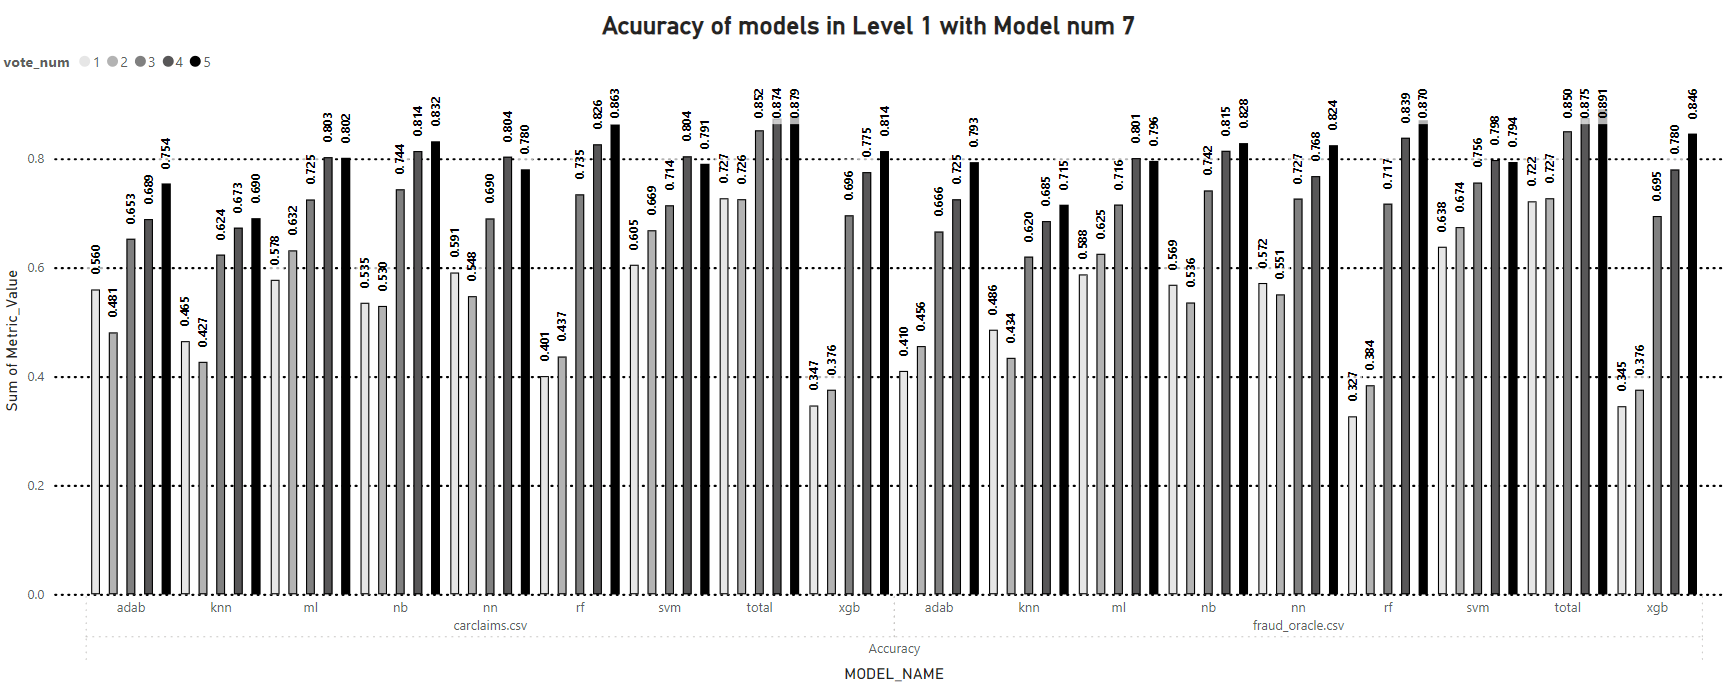
\includegraphics[scale=0.45]{Pictures/Plots-7.png}
	%% Use \caption command for figure caption and label.
	\caption{this plot as for accuracy metrics and level is 1 and model num is fixed on 7}\label{fig1}
	%% https://en.wikibooks.org/wiki/LaTeX/Importing_Graphics#Importing_external_graphics
\end{figure}



\begin{figure}[t]
	\centering%% For centre alignment of image.
	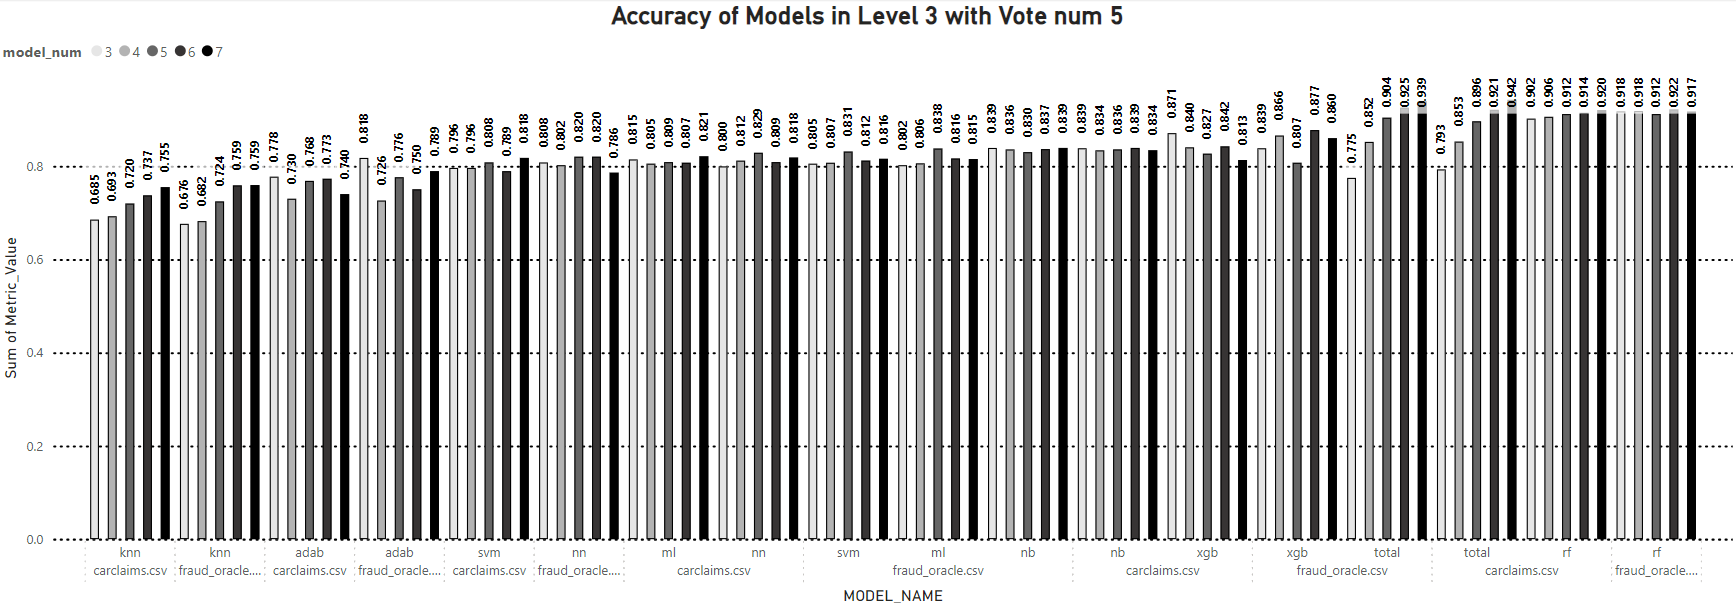
\includegraphics[scale=0.45]{Pictures/Plots-8.png}
	\caption{this plot as for accuracy metrics and level is 3 and Vote num is fixed on 5}\label{fig2}
\end{figure}

\begin{figure}[t]
	\centering%% For centre alignment of image.
	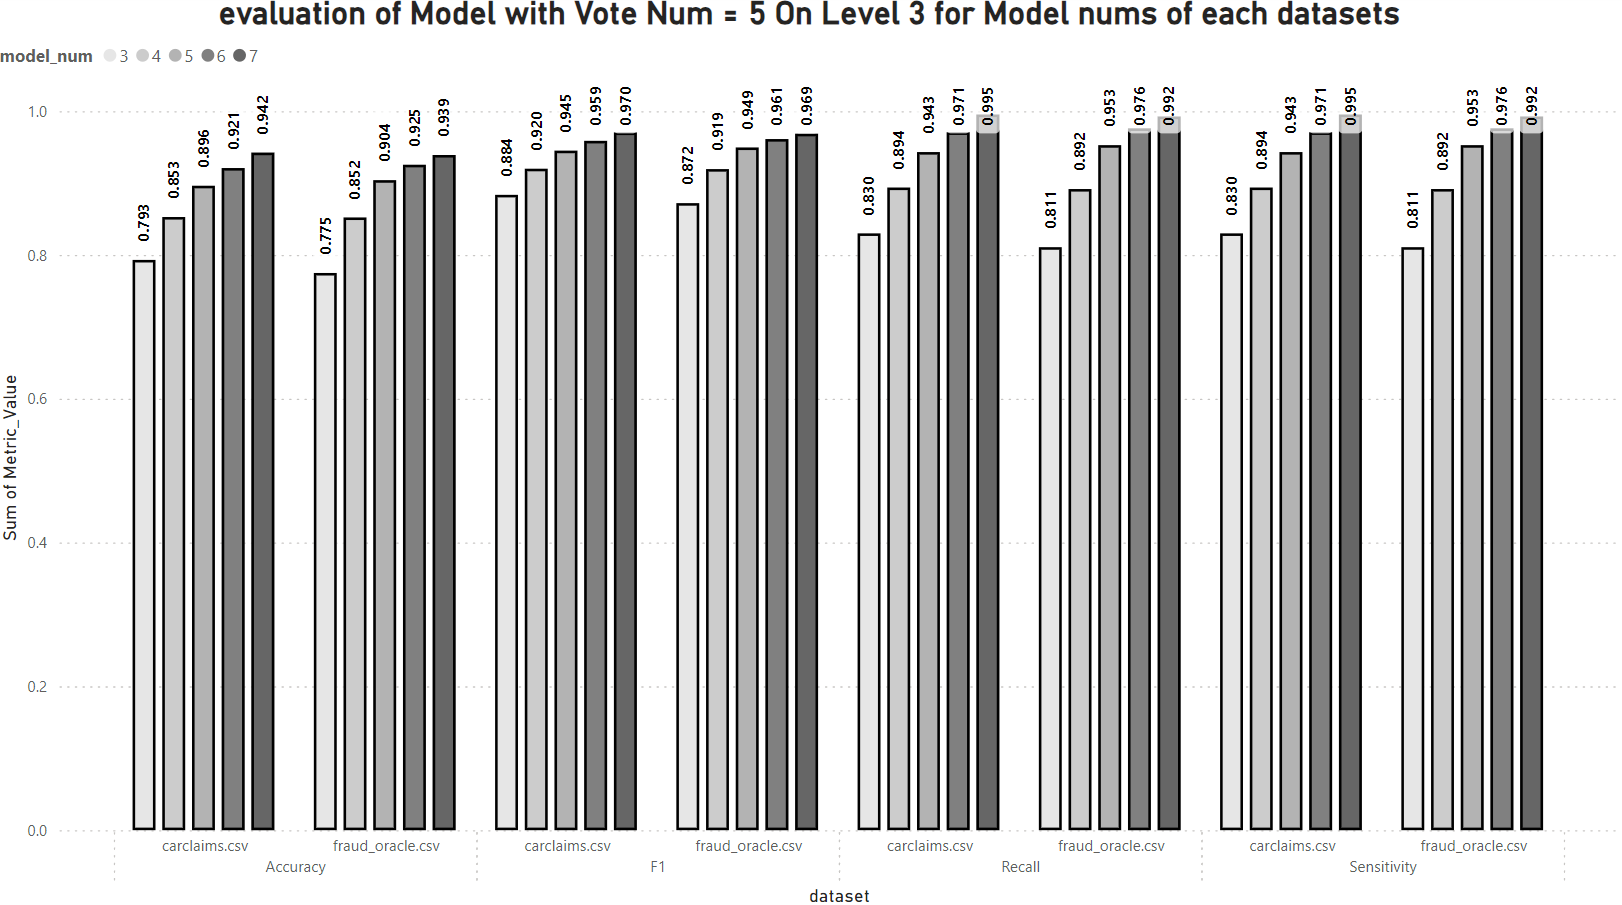
\includegraphics[scale=0.5]{Pictures/Plots-9.png}
	\caption{evaluation of Model with Vote Num = 5  On Level 3 for Model nums of each datasets}\label{fig3}
\end{figure}



\begin{figure}[t]
	\centering%% For centre alignment of image.
	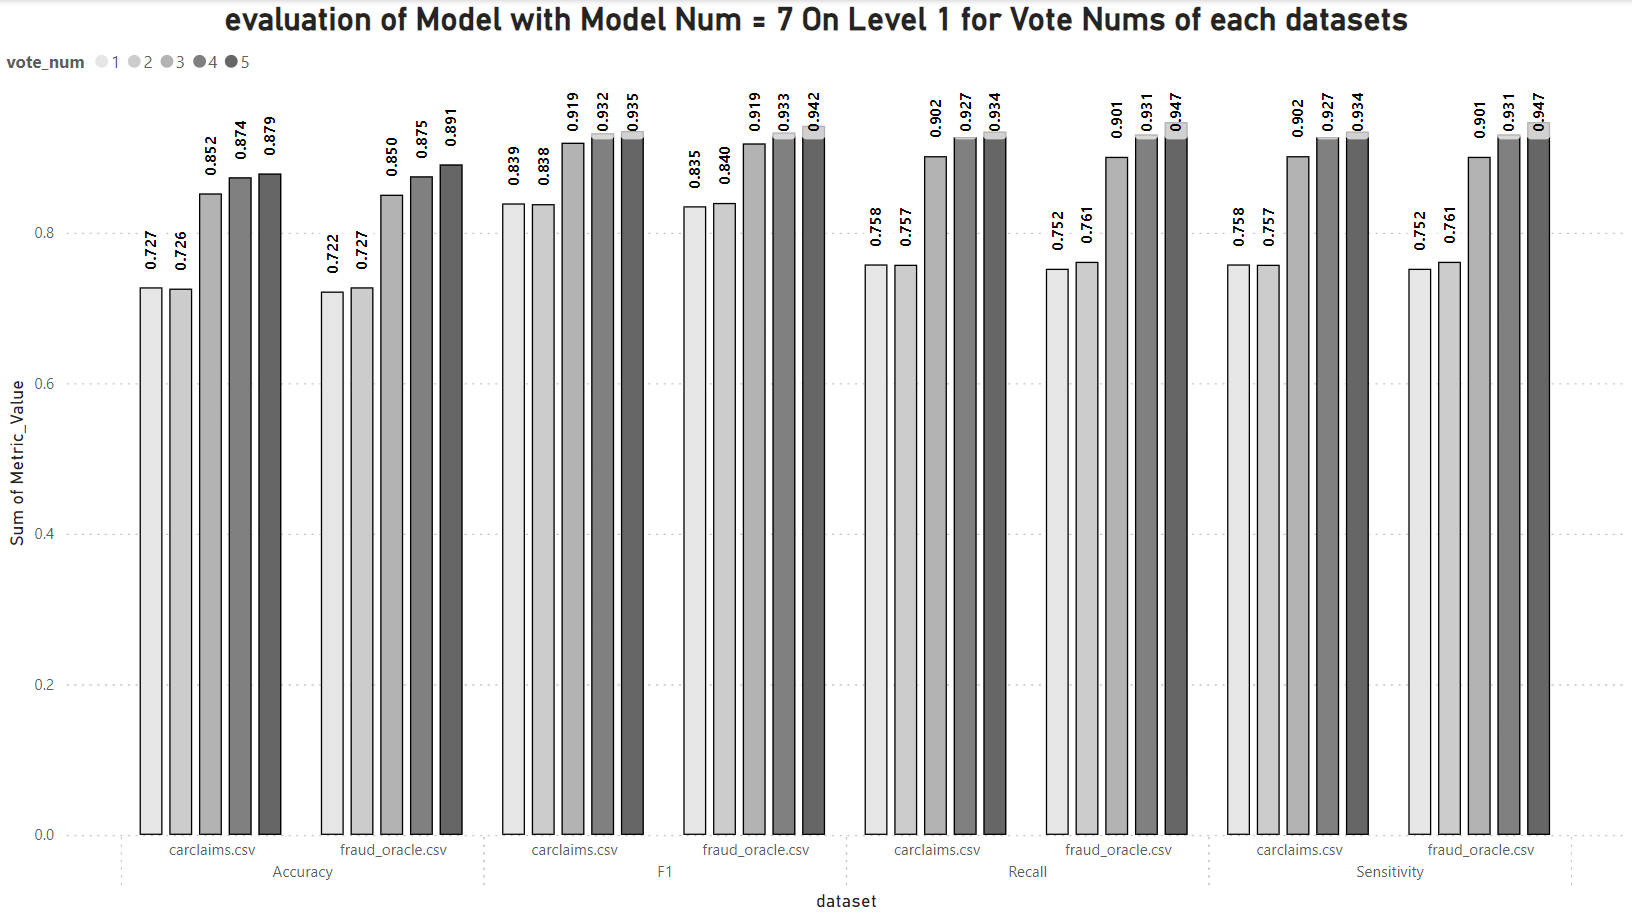
\includegraphics[scale=0.5]{Pictures/Plots-10.png}
	\caption{evaluation of Model with Model Num = 7  On Level 1 for Vote Nums of each datasets}\label{fig4}
\end{figure}
evaluation of Model with Model Num = 7  On Level 1 for Vote Nums of each datasets

CONCLUSIONS
\section{CONCLUSIONS}
\label{sec7}
in this section i will tell about the conclustions of article.


%% For citations use: 
%%       \cite{<label>} ==> [1]

%%

%%
Example citation, See \cite{lamport94}.

%% If you have bib database file and want bibtex to generate the
%% bibitems, please use
%%
%%  \bibliographystyle{elsarticle-num} 
%%  \bibliography{<your bibdatabase>}

%% else use the following coding to input the bibitems directly in the
%% TeX file.

%% Refer following link for more details about bibliography and citations.
%% https://en.wikibooks.org/wiki/LaTeX/Bibliography_Management

\end{document}

\endinput
%%
%% End of file `elsarticle-template-num.tex'.
